\documentclass{beamer}

\usepackage{paratype}
\setbeamerfont{frametitle}{family=\bf}

% Beamer theme settings
\usecolortheme{seagull}
\usenavigationsymbolstemplate{} % no navigation buttons

\usepackage[utf8]{inputenc}

\usepackage{graphicx}
\usepackage{epic}

\usepackage{amsmath}
\usepackage{amssymb}
\usepackage{amsthm}

\newcommand{\basetop}[1]{\vtop{\vskip-1ex\hbox{#1}}}
\newcommand{\source}[1]{\let\thefootnote\relax\footnotetext{\scriptsize\textcolor{kugray1}{Source: #1}}}

% for coloured code citation in text:
\usepackage{fancyvrb}

%%%%%%%%%%%%%%%%%%%%%%%%%%%%%%%%%
%%%%%    code sections   %%%%%%%%
%%%%%%%%%%%%%%%%%%%%%%%%%%%%%%%%%

% code highlighting commands in own block
\DefineVerbatimEnvironment{code}{Verbatim}{fontsize=\scriptsize}
\DefineVerbatimEnvironment{icode}{Verbatim}{fontsize=\scriptsize}

% Fancy code with color commands:
\DefineVerbatimEnvironment{colorcode}%
        {Verbatim}{fontsize=\scriptsize,commandchars=\\\{\}}

%%%%%%%%%%%%%%%%%%%%%%%%%%%%%%%%%%
%%%%%    some coloring    %%%%%%%%

\definecolor{Red}{RGB}{220,50,10}
\definecolor{Blue}{RGB}{0,51,102}
\definecolor{Yellow}{RGB}{102,51,0}
\definecolor{Orange}{RGB}{178,36,36}
\definecolor{Grey}{RGB}{180,180,180}
\definecolor{Green}{RGB}{20,120,20}
\definecolor{Purple}{RGB}{160,50,100}
\newcommand{\red}[1]{\textcolor{Red}{{#1}}}
\newcommand{\blue}[1]{\textcolor{Blue}{{#1}}}
\newcommand{\yellow}[1]{\textcolor{Yellow}{{#1}}}
\newcommand{\orange}[1]{\textcolor{Orange}{{#1}}}
\newcommand{\grey}[1]{\textcolor{Grey}{{#1}}}
\newcommand{\green}[1]{\textcolor{Green}{{#1}}}
\newcommand{\purple}[1]{\textcolor{Purple}{{#1}}}

% use "DIKU green" from our color theme for \emph
%\renewcommand{\emph}[1]{\textcolor{structure}{#1}}
\renewcommand{\emph}[1]{\textcolor{CosGreen}{ #1}}
% use some not-too-bright red for an \emp command
\definecolor{DikuRed}{RGB}{130,50,32}
\newcommand{\emp}[1]{\textcolor{DikuRed}{ #1}}
\definecolor{CosGreen}{RGB}{10,100,70}
\newcommand{\emphh}[1]{\textcolor{CosGreen}{ #1}}
\definecolor{CosBlue}{RGB}{55,111,122}
\newcommand{\emphb}[1]{\textcolor{CosBlue}{ #1}}
\definecolor{CosRed}{RGB}{253,1,1}
\newcommand{\empr}[1]{\textcolor{CosRed}{ #1}}

\newcommand{\mymath}[1]{$ #1 $}
\newcommand{\myindx}[1]{_{#1}}
\newcommand{\myindu}[1]{^{#1}}


\title{OpenCL Day 2: Loop Reasoning, Optimizing Temporal and Spatial Locality}

\author{Cosmin Oancea and Troels Henriksen}

\date{January 30, 2019}

\begin{document}

\frame{\titlepage}

\section{Content of Day2 Lecture:}

\begin{frame}
  \tableofcontents
\end{frame}

\section{Dependence Analysis}

\subsection{Problem Statement, Dependency Definition}
% slide 1
\begin{frame}[fragile,t]
  \frametitle{Problem Statement}

%[fontsize=\small]
\begin{block}{Three Loop Examples}
\begin{colorcode}
DO i = 1, N            DO i = 2, N               DO i = 2, N
 DO j = 1, N            DO j = 2, N               DO j = 1, N 
   A[j,i] = A[j,i] ..     A[j,i] = A[j-1,i-1]...   A[i,j] = ...
 ENDDO                    B[j,i] = B[j-1,i]...       A[i-1,j+1]
ENDDO                  ENDDO ENDDO               ENDDO ENDDO
\end{colorcode}
\end{block} 

Iterations are ordered {\em lexicographically}, in the order
they occur in the sequential execution: 
{\tt$\vec{k}=$(i=2,j=4) < $\vec{l}=$(i=3,j=3)}.

\bigskip

\begin{itemize}
    \item \emp{Which of the three loop nests is amenable to parallelization?}\smallskip
    \item Loop interchange is one of the most simple and useful code transformations,
            e.g., used to enhance locality of reference, and even to ``create'' 
            parallelism.\smallskip
    \item \emp{In which loop nest is it safe to interchange the loops?}
\end{itemize}

\end{frame}

% slide 2
\begin{frame}[fragile,t]
  \frametitle{Definition of a Dependency} % of CPU, Multicores, GPGPU
\vspace{-2ex}
\begin{block}{Load-Store Classification of Dependencies}
\begin{colorcode}
True Dependency(RAW)  Anti Dependency(WAR)  Output dependency(WAW)
   S1    X  = ..         S1    .. = X          S1    X = ...            
   S2    .. = X          S2    X  = ..         S2    X = ...
\end{colorcode}
\end{block} 

\smallskip

{\bf Def. Loop Dependence:} There is a dependence from statement $S1$ to $S2$
in a loop nest {\em iff} there exist iterations $\vec{k} \leq \vec{l}$ and
an execution path from statement $S1$ to statement $S2$ \emp{such that:}
\begin{description}
    \item[1.] $S1$ accesses memory location $M$ on iteration $\vec{k}$, and
    \item[2.] $S2$ accesses memory location $M$ on iteration $\vec{l}$, and
    \item[3.] one of these accesses is a write.
\end{description}
\medskip

\emp{We say that $S1$ is the source and $S2$ is the sink of the dependence}, 
because $S1$ executes before $S2$ in the sequential program execution.
Dependence depicted with an arrow pointing from source to sink.\pause

\medskip
\emp{We are most interested in cross iteration dependencies, i.e., $\vec{k} < \vec{l}$.}

\end{frame}

\begin{frame}[fragile,t]
  \frametitle{Loop-Nest Dependencies} % of CPU, Multicores, GPGPU

{\em Lexicographic ordering}, 
e.g., {\tt$\vec{k}=$(i=2,j=4) < $\vec{l}=$(i=3,j=3)}.

%[fontsize=\small]
\begin{block}{Three Loop Examples}
\begin{colorcode}
DO i = 1, N            DO i = 2, N               DO i = 2, N
 DO j = 1, N            DO j = 2, N               DO j = 1, N 
   A[j,i] = A[j,i] ..     A[j,i] = A[j-1,i-1]...   A[i,j] = ...
 ENDDO                    B[j,i] = B[j-1,i]...       A[i-1,j+1]
ENDDO                  ENDDO ENDDO               ENDDO ENDDO
\end{colorcode}
\end{block} 
\pause

\hspace{-5ex}\includegraphics[height=20ex]{img/day2/LoopDeps}  

\emp{How can I summarize this information?} %Do I have to consider all cases?
\end{frame}

\subsection{Dependency Matrix, Loop Parallelism and Interchange}
\begin{frame}[fragile,t]
  \frametitle{Aggregate Dependencies via Direction Vectors} % of CPU, Multicores, GPGPU

\begin{block}{Three Loop Examples}
\begin{colorcode}
DO i = 1, N            DO i = 2, N               DO i = 2, N
 DO j = 1, N            DO j = 2, N               DO j = 1, N 
   A[j,i] = A[j,i] ..     A[j,i] = A[j-1,i-1]...   A[i,j] = ...
 ENDDO                    B[j,i] = B[j-1,i]...       A[i-1,j+1]
ENDDO                  ENDDO ENDDO               ENDDO ENDDO
\end{colorcode}
\end{block} 

\smallskip

Dependencies depicted via an edge {\em from} the stmt that executes first
in the loop nest ({\em source}), {\em to} the one that executes later ({\em sink}).

\smallskip

{\bf Def. Dependence Direction:} Assume there exists a dependence from $S1$
in iteration $\vec{k}$ to $S2$ in $\vec{l}$ ($\vec{k}\leq\vec{l}$). 
\emp{\em The direction vector is}:
\begin{description}
    \item[1.] $\vec{D}(\vec{k},\vec{l})_m = $~``{\tt{}<}'' if $\vec{k}_m < \vec{l}_m$,
    \item[2.] $\vec{D}(\vec{k},\vec{l})_m = $~``{\tt{}=}'' if $\vec{k}_m = \vec{l}_m$,
    \item[3.] $\vec{D}(\vec{k},\vec{l})_m = $~``{\tt{}>}'' if $\vec{k}_m > \vec{l}_m$.
    \item[4.] $\vec{D}(\vec{k},\vec{l})_m = $~``{\tt{}*}'' otherwise.
\end{description}

\medskip
If the source is a write and the sink a read then RAW dependency,\\
if the source is a read then WAR, if both are writes then WAW.  
\end{frame}

\begin{frame}[fragile,t]
  \frametitle{How to Compute the Direction Vectors?}
\begin{itemize}
    \item For any two statements $S1$ and $S2$ that may access the same
            array $A$ (and one of the accesses is a write),\medskip
    \item in two symbolic iterations $I^1\equiv(i^1_1,\ldots i^1_m)$
            and $I^2=(i^2_1,\ldots i^2_m)$ (assuming $I^1 \leq I^2$)\medskip
    \item on indices $A[e^1_1,\ldots,e^1_n]$ and $A[e^2_1,\ldots,e^2_n]$,
            respectivelly,\medskip
    \item then \textbf{\it the direction vectors may be derived} from the equations\\
            $\begin{cases}
                e^1_1 = e^2_1\\
                \ldots\\
                e^1_n = e^2_n
            \end{cases}$\\\medskip
            (The system of equations models the definition of a dependency: 
                both accesses need to refer to the same memory location!)
\end{itemize}
\end{frame}

\begin{frame}[fragile,t]
  \frametitle{When is a Loop Parallel?} % of CPU, Multicores, GPGPU

\begin{block}{Direction Vectors/Matrix for Three Loops }
\begin{columns}
\column{0.27\textwidth}
\begin{colorcode}
  DO i = 1, N
    DO j = 1, N
S1    A[j,i]=A[j,i]..
    ENDDO
  ENDDO\pause
For S1\mymath{\rightarrow}S1: 
    (j1,i1)=(j2,i2) 
    i1 \emp{=} i2 \& j1 \emp{=} j2

Direction matrix:
S1\mymath{\rightarrow}S1: \emp{[=,=]}
\end{colorcode}
\column{0.32\textwidth}
\begin{colorcode}
  DO i = 2, N
    DO j = 2, N
S1    A[j,i]=A[j-1,i]...
S2    B[j,i]=B[j-1,i-1]...
    ENDDO
  ENDDO\pause
S1\mymath{\rightarrow}S1: (j1,i1)=(j2-1,i2)
        i1 \emp{=} i2 \& j1 \emp{<} j2
S2\mymath{\rightarrow}S2: (j1,i1)=(j2-1,i2-1)
        i1 \emp{<} i2 \& j1 \emp{<} j2
S1\mymath{\rightarrow}S1: \emp{[=,<]}
S2\mymath{\rightarrow}S2: \emp{[<,<]}
\end{colorcode}
\column{0.32\textwidth}
\begin{colorcode}
  DO i = 2, N
    DO j = 1, N
S1    A[i,j]=A[i-1,j+1]...
    ENDDO
  ENDDO
For S1\mymath{\rightarrow}S1:\pause
    (i1,j1) = (i2-1,j2+1)
    i1 \emp{<} i2 \& j1 \emp{>} j2

Direction matrix:
S1\mymath{\rightarrow}S1: \emp{[<,>]}
\end{colorcode}
\end{columns}
\end{block} 

{\bf Th. Parallelism:} A loop in a loop nest is parallel {\em iff} for each entry in its direction column, the entry is either {\tt =} or there exists an outer loop whose corresponding direction is {\tt <}. 

\smallskip

\red{A direction vector cannot have $>$ as the first non-= symbol},\\
as that would mean that I depend on something in the future. 
\end{frame}

\begin{frame}[fragile,t]
  \frametitle{Parallelism and Loop Interchange} % of CPU, Multicores, GPGPU

\begin{block}{Direction Vectors/Matrix for Three Loops }
\begin{columns}
\column{0.27\textwidth}
\begin{colorcode}
  DO i = 1, N
    DO j = 1, N
S1    A[j,i]=A[j,i]..
    ENDDO
  ENDDO
For S1\mymath{\rightarrow}S1: 
    (j1,i1)=(j2,i2) 
    i1 \emp{=} i2 \& j1 \emp{=} j2

Direction matrix:
S1\mymath{\rightarrow}S1: \emp{[=,=]}
\end{colorcode}
\column{0.32\textwidth}
\begin{colorcode}
  DO i = 2, N
    DO j = 2, N
S1    A[j,i]=A[j-1,i]...
S2    B[j,i]=B[j-1,i-1]...
    ENDDO
  ENDDO
S1\mymath{\rightarrow}S1: (j1,i1)=(j2-1,i2)
        i1 \emp{=} i2 \& j1 \emp{<} j2
S2\mymath{\rightarrow}S2: (j1,i1)=(j2-1,i2-1)
        i1 \emp{<} i2 \& j1 \emp{<} j2
S1\mymath{\rightarrow}S1: \emp{[=,<]}
S2\mymath{\rightarrow}S2: \emp{[<,<]}
\end{colorcode}
\column{0.32\textwidth}
\begin{colorcode}
   DO i = 2, N
    DO j = 1, N
 S1   A[i,j] = ...
        A[i-1,j+1]
   ENDDO ENDDO
  For S1\mymath{\rightarrow}S1: 
    (i1,j1) = (i1-1,j2+1)
    i1 \emp{<} i2 \& j1 \emp{>} j2

  Direction matrix:
  S1\mymath{\rightarrow}S1: \emp{[<,>]}
\end{colorcode}
\end{columns}
\end{block} 

{\bf Th. Loop Interchange:} Interchanging two loops in a loop nest 
is legal {\em iff} interchanging the columns of the direction matrix
in the same way {\em does NOT result} in a {\tt >} direction as the
leftmost non-{\tt{}=} direction in a row. 
\end{frame}


\begin{frame}[fragile,t]
  \frametitle{Parallelism and Loop Interchange} 

\begin{block}{Direction Vectors/Matrix for Three Loops }
\begin{colorcode}
  DO i = 1, N           DO i = 2, N             DO i = 2, N
    DO j = 1, N          DO j = 2, N             DO j = 1, N 
S1    A[j,i]=A[j,i]..  S1  A[j,i]=A[j-1,i]...   S1 A[i,j]=A[i-1,j+1]...
    ENDDO              S2  B[j,i]=B[j-1,i-1]...  ENDDO
  ENDDO                 ENDDO ENDDO             ENDDO

For S1\mymath{\rightarrow}S1: j1 = j2    For S1\mymath{\rightarrow}S1: j1 = j2-1   For S1\mymath{\rightarrow}S1: i1 = i2-1
            i1 = i2                i1 = i2                j1 = j2+1
(i2,j2)-(i1,j1)=         (i2,j2)-(i1,j1)=\emp{[=,<]}  (i2,j2)-(i1,j1)=
\emp{[=,=]}                  For S2\mymath{\rightarrow}S2: j1 = j2-1        \emp{[<,>]}
                                   i1 = i2-1
                         (i2,j2)-(i1,j1)=\emp{[<,<]}
\end{colorcode}
\end{block} 

Interchange is safe for the 1st and 2nd nests, but not for the 3rd!\\
e.g., \emp{\tt [=,<]}$~~~\rightarrow~~~$ \emph{\tt [<,=]}$~~~~~~~~~$(for the second loop nest)\\
$~~~~~~~$\emp{\tt [<,<]}$~~~~~~~~~~~~~$\emph{\tt [<,<]}

\pause\smallskip

After interchange, loop $j$ of the second loop nest is parallel.

\bigskip

\emph{\bf Corollary: A parallel loop can be always interchanged inwards.}
\end{frame}

\subsection{Loop Distribution, Array Expansion/Privatization}
\begin{frame}[fragile,t]
  \frametitle{Dependency Graph and Loop Distribution} 

{\bf Def. Dependency Graph:} edges from the source of the dependency, i.e., early iteration, 
to the sink, i.e., later iteration. 

\smallskip

{\bf Th. Loop Distribution:} Statements that are in a dependence cycle remain in one 
(sequential) loop.   The others are distributed to separate loops in graph order; 
if no cycle then parallel loops.\smallskip

\begin{block}{Vectorization Example}
\begin{columns}
\column{0.34\textwidth}
\begin{colorcode}[fontsize=\scriptsize]
  DO i = 3, N
\emp{S1  A[i] = B[i-2] ...}
\red{S2  B[i] = B[i-1] ...}
  ENDDO  

For S2\mymath{\rightarrow}S1: i1 = i2-2, \emp{[<]}
For S2\mymath{\rightarrow}S2: i1 = i2-1, \emp{[<]}
\end{colorcode}
\column{0.27\textwidth}\pause
\includegraphics[height=12ex]{img/day2/LoopDistr}  
\column{0.30\textwidth}
\begin{colorcode}[fontsize=\scriptsize]
  \red{DO} i = 3, N
S2  B[i] = B[i-1] ...
  \red{ENDDO}

  \emphh{DOALL} i = 3, N
\emp{S1  A[i] = B[i-2] ...}
  \emphh{ENDDOALL}
\end{colorcode}
\end{columns}
\end{block}

\medskip

{\bf Corollary:} It is always legal to distribute a parallel loop;\\
\red{but requires array expansion for local variables or if output
dependencies are present.}
\end{frame}

\begin{frame}[fragile,t]
  \frametitle{Loop Distribution May Require Array Expansion} 

\begin{columns}
\column{0.4\textwidth}
\begin{colorcode}[fontsize=\scriptsize]
  float tmp;
  for(i=2; i<N; i++) \{
    \emp{tmp} = 2*B[i-2]; 
    A[i] = tmp;
    B[i] = tmp+B[i-1]
  \}
\end{colorcode}
\column{0.53\textwidth}
\begin{colorcode}[fontsize=\scriptsize]
  \emph{float tmp[N]};
  for(int i=2; i<N; i++) \{
    tmp[i] = 2*B[i-2]; 
    B[i] = tmp[i]+B[i-1];
  \}

  \emph{forall(int i=2; i<N; i++)} \{
    A[i] = tmp[i];
  \}
\end{colorcode}
\end{columns}
\bigskip

No matter where {\tt tmp} is declared (inside or outside
the loop) it needs to be expanded into an array in order
to do loop distribution.\bigskip

If {\tt tmp} is declared outside the loop then requires \emp{\bf privatization}, \pause
because it actually causes frequent {\sc waw} dependencies.
However its value is written before being used within the same iteration.
Hence it is semantically equivalent to a locally declared variable,
which will remove the output ({\sc waw}) dependency.\bigskip

Distribution requires array expansion of the scalar {\tt tmp}.

\end{frame}

\begin{frame}[fragile,t]
  \frametitle{False Dependencies (WAR/WAW)} 

\begin{itemize}
    \item \emp{Cross-Iteration Anti Dependencies (WAR)} 
        correspond to a read from the array as it was 
        before the loop $\Rightarrow$ can be eliminated
        by reading from a copy of the array.\bigskip

    \item \emp{Cross-Iteration WAW Dependencies (WAW)}:\\
        If they correspond to the case in which every \emp{\bf read} from
        a scalar or array location is covered by a \emp{\bf previous same-iteration write}
        %a re-writing the same array elements
        %in different iterations 
        $\Rightarrow$ can be eliminated \emph{\bf privatization (renaming)},
        which semantically moves the declaration of the variable (scalar or array) 
        inside the loop.\bigskip

    \item Direction-vectors reasoning is limited to relatively
        simple loop nests, e.g., difficult to reason about 
        privatization in such a way.
\end  {itemize}
\end{frame}

\begin{frame}[fragile,t]
  \frametitle{Example: Eliminating WAW Dependencies} 

\begin{columns}
\column{0.40\textwidth}
\begin{colorcode}[fontsize=\scriptsize]
  \emp{float A[M];}
  \emp{for}(i=0; i<N; i++)\{
    for(int j=0, j<M; j++)
        \emp{A[j]} = (4*i+4*j) \% M;
    for(int k=0; k<N; k++)
        X[i][k] = X[i][k-1] * 
           \emp{A[A[(2*i+k)\%M]\%M]};
  \}\pause
\end{colorcode}

\column{0.58\textwidth}
\begin{colorcode}[fontsize=\scriptsize]
  // \emp{The write to A[j] causes many WAWs},\pause
  // \emph{but A is fully written in loop j}
  // \emph{float A[N][M];}
  \emph{forall}(int i=0; i<N; i++)\{
    \emph{float A[M];}
    for(int j=0, j<M; j++)
        \emph{A[j]} = (4*i+4*j) \% M; // \emph{A[i][j]}
    for(int k=0; k<N; k++)
        X[i][k]=X[i][k-1] * 
           \emph{A[A[(2*i+k)\%M]\%M]};
           //\emph{A[i][A[i,...]]}
  \}
\end{colorcode}
\end{columns}

For OpenCL programming you would likely use array expansion (\emph{\tt float A[N,M]})
because the size {\tt M} is likely unknown at compile time.\smallskip

\end{frame}

\subsection{Exercise: Putting it all together}

\begin{frame}[fragile,t]
  \frametitle{Putting Everything Together} 

\begin{colorcode}[fontsize=\scriptsize]
float X[M][N][N]; /* ... compute X ... */
float A[N][N];
for(int i = 0; i < M; i++) \{
  \emp{//initialize A}
  for(int k = 0; k < N; k++) \{
    for(int j = 0; j < N; j++) \{
        float x = X[i][j][k];
        A[k][j] = x * x;
  \} \}
  \emp{// convergence loop}
  for(int t = 0; t < T; t++) \{
    for(int j = 0; j < N; j++) \{
      for(int k = 0; k < N; k++) \{
        A[k][j] = fsqrt(A[k][j] * A[k-1][j]);
        X[i][k][j] += fsqrt(B[i][k-1][j-1]);
      \}
    \}
\} \}
\end{colorcode}

{\bf Exercise:} 
Assume the code above runs on a dataset having\\
{\tt M = 128} and {\tt N = 512} and, less important, say {\tt T = 256}.\\\smallskip
\begin{itemize}
    \item[(1)] Is this code suitable for GPU execution?\\\smallskip
    \item[(2)] Transform the code to one suitable for GPU execution.
\end{itemize}
\end{frame}

%%%%%%%%%%%%%%%%%%%%%%%%%%%%%%%%%%%%%%%%%%%%%%%%%%%%%%%%
%%% Spatial Locality
%%%%%%%%%%%%%%%%%%%%%%%%%%%%%%%%%%%%%%%%%%%%%%%%%%%%%%%%

\section{Optimizing Spatial Locality (Coalesced Memory)}

\begin{frame}[fragile]
	\tableofcontents[currentsection]
\end{frame}

\subsection{Motivating Example on A Contrived Program}

\begin{frame}[fragile,t]
  \frametitle{Motivation: Coalesced Accesses to Global Memory} 

Which are the parallel/sequential loops?

\begin{columns}
\column{0.42\textwidth}
\begin{colorcode}[fontsize=\scriptsize]
real A[height][width];
real B[height][width];
// Non-Coalesced Access
\emph{for(i=0; i<height; i++) \{}
  real accum  = 0.0;

  \emp{for(j=0; j<width; j++) \{}
    real tmpA = A[i][j];
    accum = tmpA*tmpA - accum;
    B[i][j] = accum;
  \}
\}\pause
\end{colorcode}
\column{0.55\textwidth}
\begin{colorcode}[fontsize=\scriptsize]
A' = transpose(A);
// Coalesced Accesses
\emph{for(i=0; i<height; i++) \{}
  real accum = 0.0;

  \emp{for(int j=0; j<width; j++) \{}
    real tmpA = A'[j][i];
    accum = tmpA*tmpA - accum;
    B'[j][i] = accum;
  \}
\}
B = transpose(B');
\end{colorcode}
\end{columns}
\bigskip

\begin{itemize}
    \item \emph{Loop {\tt i} is parallel;}\smallskip
    \item \emp{loop {\tt j} is sequential} because 
            of the RAW cross-iteration dependencies on {\tt accum}.\bigskip
    \item The transformed program performs about $3\times$ the number
            of global-memory accesses than the original. \pause\smallskip
    \item But it is significantly faster than the original (on GPUs).
\end{itemize}

\end{frame}

\begin{frame}[fragile,t]
  \frametitle{Motivation: What Are Coalesced Accesses?} 

\textbf{Coalesced access}: a (quarter) wave accesses in a
SIMD instruction consecutive words in global-memory.\bigskip

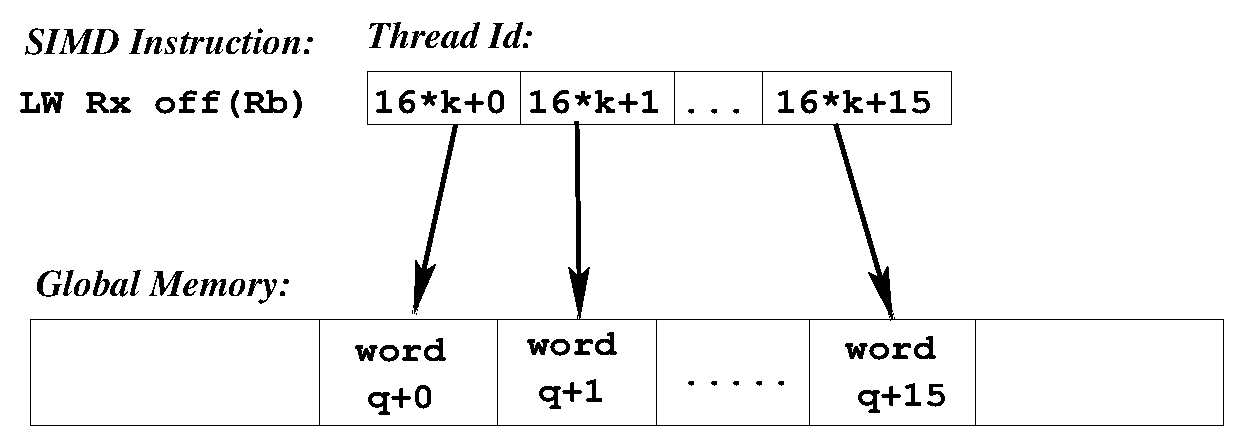
\includegraphics[height=20ex]{img/day2/CoalescedGPU}

\end{frame}

\subsection{Uncoalesced Matrix Transposition Kernel}

\begin{frame}[fragile,t]
  \frametitle{Uncoalesced Transposition Kernel} 

\begin{itemize}
    \item Semantically we chunk the matrix into {\tt T$\times$T} blocks;
    \item Each block is processed by one workgroup, e.g., {\tt T=16}.
\end{itemize}

\begin{columns}
\column{0.40\textwidth}
\begin{colorcode}[fontsize=\scriptsize]
// Initial
for(i=0; i<height; i++) \{    
  for(j=0; j<width; j++) \{ 
    B[j*height+i] =
           A[i*width+j];
  \}
\}
\end{colorcode}
\column{0.58\textwidth}
\begin{colorcode}[fontsize=\scriptsize]
// Blocked
\emp{for(ii=0; ii<height; ii+=T) \{}
  \emp{for(jj=0; jj<width; jj+=T) \{}
    \emphh{for(i=ii; i<min(ii+T,height); i++) \{}
      \emphh{for(j=jj; j<min(jj+T,width); j++) \{}
        \red{B[j*height+i]} = A[i*width+j];
\} \} \} \}
\end{colorcode}
\end{columns}

\begin{itemize}
\item Local workgroup: $T\times T$; 
\item Global(1): $\lceil \texttt{width}/T \rceil * T$; Global 1: $\lceil \texttt{height}/T \rceil * T$.
\end{itemize}
\pause

\begin{colorcode}[fontsize=\scriptsize]
__kernel void naiveTransp( __global real* A, __global real* B
                         , int height, int width ) \{
    unsigned int i = get_global_id(1);
    unsigned int j = get_global_id(0); 
    if( (j >= width) || (i >= height) ) return;
    \red{B[j*height + i]} = A[i*width + j];  \red{// uncoalesced access!}
\}

\end{colorcode}

\end{frame}

\subsection{Coding Exercise: Entirely-Coalesced Transposition}

\begin{frame}[fragile,t]
  \frametitle{Exercise 1: Fill In Coalesced Transposition Kernel} 
\vspace{-1ex}
\begin{colorcode}[fontsize=\scriptsize]
// verifies that workgroup size is: TILE*TILE
__kernel __attribute__((reqd_work_group_size(TILE, TILE, 1)))
__kernel void coalsTransp( __global real* A, 
        __global real* B, uint32_t height, uint32_t width ) \{
  __local float tile[TILE][TILE];                    \red{// local memory}
  int gidx = get_global_id(0); int gidy = get_global_id(1);
  int lidx = get_local_id(0);  int lidy = get_local_id(1);

  // 1. read current element from global to local memory.
  //    make sure to NOT access arrays out of bounds!
  // 2. current thread loads from local memory the transposed element
  //    at workgroup level, and writes it in the proper position in B.
  //    Useful functions: get_group_id(0), get_local_size(0); or 1.
  // 3. Insert necessary workgroup-level synchronization
  //    barrier(CLK_LOCAL_MEM_FENCE);
\}
\end{colorcode}

Transposing a (blocked) matrix $\equiv$ moving each block to 
the transposed position $+$ transposing each block!\medskip

\pause
\begin{itemize}
    \item \emp{Implement in {\tt Day2-Exercises/Transp/kernels.cl}}
    \item Are the read and write accesses to global memory coalesced?
    \item Why/Where should you place the barrier?
\end{itemize}

\end{frame}

%\begin{frame}[fragile,t]
%  \frametitle{Coalesced Transposition Kernel} 
%
%\begin{colorcode}[fontsize=\scriptsize]
%__kernel void coalsTransp coalsTransp( __global real* A, 
%        __global real* B, uint32_t height, uint32_t width ) \{
%  __local float tile[T][T];                          \red{// local memory}
%  int gidx = get_global_id(0); int gidy = get_global_id(1);
%  int lidx = get_local_id(0);  int lidy = get_local_id(1);
%
%  if( gidx < width && gidy < height )          \red{// cannot return here!}
%    lmem[lidy*T + lidx] = A[gidy*width + gidx]; \red{// copy to local mem!}
%  \red{barrier(CLK_LOCAL_MEM_FENCE); // all threads have to reach barrier!}
%
%  gidx = get_group_id(1)*T + lidx; gidy = get_group_id(0)*T + lidy;
%  if( gidx < height && gidy < width )
%      B[gidy*height + gidx] = lmem[lidx*T + lidy];
%\}
%\end{colorcode}
%
%\end{frame}


\subsection{Program Optimized By Transposition + Coding Exercise}

\begin{frame}[fragile,t]
  \frametitle{Exercise 2: Coalescing By Transposition} 

\begin{columns}
\column{0.42\textwidth}
\begin{colorcode}[fontsize=\scriptsize]
real A[height][width];
real B[height][width];
// Non-Coalesced Access
\emph{for(i=0; i<height; i++) \{}
  real accum  = 0.0;

  \emp{for(j=0; j<width; j++) \{}
    real tmpA = A[i][j];
    accum = tmpA*tmpA - accum;
    B[i][j] = accum;
\} \}\pause
\end{colorcode}
\column{0.55\textwidth}
\begin{colorcode}[fontsize=\scriptsize]
A' = transpose(A);
// Coalesced Accesses
\emph{for(i=0; i<height; i++) \{}
  real accum = 0.0;

  \emp{for(int j=0; j<width; j++) \{}
    real tmpA = A'[j][i];
    accum = tmpA*tmpA - accum;
    B'[j][i] = accum;
\} \}
B = transpose(B');
\end{colorcode}
\end{columns}
\bigskip

\begin{itemize}
    \item Open File "Day2-Exercises/Transp/coalescing.c", function named "runGPUcoalsProgram".
    \item Fill the correct sizes for the "coalsProgrm" kernel call.
    \item Open File "Day2-Exercises/Transp/kernels.cl" and implement kernel named "coalsProgrm".
    \item Fix bugs until it validates! :-)
    \item What is the speedup with respect to the naive program?
    \item What fraction of the memcpy bandwidth is achieved? 
\end{itemize}


\end{frame}

\subsection{Fully Fused Program + Coding Exercise}

\begin{frame}[fragile,t]
  \frametitle{Exercise 3: Fused Program With Coalesced Accesses}

\begin{itemize}
    \item Open File "Day2-Exercises/Transp/kernels.cl" and implement the missing pieces from kernel named "optimProgrm";\bigskip
    \item The idea is to have coalesced accesses "fused" into the kernel by each 
            thread processing {\tt CHUNK} elements at a time by:\smallskip
    \begin{itemize}
        \item collectively copying {\tt CHUNK * WORKGROUP\_SIZE} input elements from global to local memory
                in coalesced fashion;\smallskip
        \item each thread now processes {\tt CHUNK} elements from its row;\smallskip
        \item collectively copying {\tt CHUNK * WORKGROUP\_SIZE} result elements from local to global memory
                in coalesced fashion;\smallskip
        \item repeat in a loop (inside the kernel) until all row's elements have been processed! 
    \end{itemize}\bigskip
    \item Fix bugs until it validates! :-)\bigskip
    \item What is the speedup with respect to the transposition-optimized program?\bigskip
    \item What fraction of the memcpy bandwidth is achieved? 
\end{itemize}


\end{frame}


%%%%%%%%%%%%%%%%%%%%%%%%%%%%%%%%%%%%%%%%%%%%%%%%%%%%%%%%
%%% Temporal Locality
%%%%%%%%%%%%%%%%%%%%%%%%%%%%%%%%%%%%%%%%%%%%%%%%%%%%%%%%
\section{Optimizing Temporal Locality}

\begin{frame}[fragile]
	\tableofcontents[currentsection]
\end{frame}

\subsection{Naive Matrix-Matrix Multiplication}

\begin{frame}[fragile,t]
  \frametitle{Matrix Multiplication: Loop Strip Mining}

\begin{columns}
\column{0.64\textwidth}
\begin{colorcode}[fontsize=\scriptsize]
for (int i = 0; i < M; i++) \{  \emphh{// Parallel}
  for (int j = 0; j < N; j++) \{  \emphh{// Parallel}
    float tmp = 0.0
    for(int k = 0; k < U; k++) \{ \emp{// Reduction}
      tmp += A[i,k]*B[k,j] 
    \}
    C[i,j] = tmp;          
  \}
\}
\end{colorcode}
\column{0.33\textwidth}
Matrices:
\begin{itemize}
    \item {\tt A $\in~\mathcal{M}^{M \times U}$}
    \item {\tt B $\in~\mathcal{M}^{U \times N}$}
    \item {\tt C$\in~\mathcal{M}^{M \times N}$} 
\end{itemize}
Loops of indices {\tt i} and {\tt j} are parallel.
\end{columns}

\bigskip

Accesses to {\tt A} and {\tt B} invariant to loops {\tt i} and {\tt j} $\Rightarrow$\\
\emph{The idea is to apply Block Tiling to optimize temporal locality!}  
\end{frame}

\subsection{Block-Tiled Matrix Multiplication + Coding Exercise}

\begin{frame}[fragile,t]
  \frametitle{Loop Strip Mining}

\begin{columns}
\column{0.43\textwidth}
\begin{colorcode}[fontsize=\scriptsize]
for(int i = 0; i < N; i++) \{
    loop_body(i)             \emp{\mymath{\Rightarrow}}
\}


\end{colorcode}
\column{0.56\textwidth}
\begin{colorcode}[fontsize=\scriptsize]
for(int ii = 0; ii < N; ii += T) \{        \alert{// for some tile T}
  for(int i = ii; i<MIN(ii+T,N); i++) \{ 
    loop_body(i)
\}  \}
\end{colorcode}
\end{columns}

\emph{Strip Mining is always safe:} the transformed loop executes
the same instructions in the same order as the original loop!
\bigskip

Strip mining all loops by some tile {\tt T} result in:\pause\smallskip

\begin{colorcode}[fontsize=\scriptsize]
for (int ii = 0; ii < M; ii += T) \{            \emphh{// Parallel}
  for (int i = ii; i < MIN(ii+T,M); i++) \{     \emphh{// Parallel}
    for (int jj = 0; jj < N; jj += T) \{        \emphh{// Parallel}
      for (int j = jj; j < MIN(jj+T,N); j++) \{ \emphh{// Parallel}
          float tmp = 0.0;
          for(int kk = 0; kk < U; k += T) \{    \emp{// Reduction}
            for(int k=kk; k<MIN(kk+T,U); k++) \{\emp{// Reduction}
                tmp += A[i,k]*B[k,j];
            \}
          \}
          C[i,j] = tmp;          
      \}
    \}
  \}
\}
\end{colorcode}
\end{frame}

\begin{frame}[fragile,t]
  \frametitle{Block Tiling: Strip Mining + Interchange}

\emph{Now interchange the loops if index {\tt i} and {\tt jj}.} Why is this safe?\smallskip

\begin{colorcode}[fontsize=\scriptsize]
for (int ii = 0; ii < M; ii += T) \{             \emp{// Global 1}
  for (int jj = 0; jj < N; jj += T) \{           \emp{// Global 0}
    for (int i = ii; i < MIN(ii+T,M); i++) \{    \emphh{// Local 1}
      for (int j = jj; j < MIN(jj+T,N); j++) \{  \emphh{// Local 0}
          float tmp = 0.0;
          for(int kk = 0; kk < U; k += T) \{     \emp{// Sequential}

            \red{//What slices of A and B are used in the loop below?}

            for(int k=kk; k<MIN(kk+T,U); k++) \{ \emp{// Sequential}
                tmp += A[i,k]*B[k,j];
            \}
          \}
          C[i,j] = tmp;          
\} \} \} \}
\end{colorcode}

\pause

\emph{\tt A[ii : MIN(ii+T,M)][kk : MIN(kk+T,U)]}\\
\emph{\tt B[kk : MIN(kk+T,U)][jj : MIN(jj+T,N)]}\\\smallskip

Each array slice has {\tt T$\times$T} elements and there are {\tt T$\times$T} threads in a workgroup;
so each thread can copy one element to local memory.\\  
Thus, we cut the number of global-memory accesses by a {\tt T} factor.

\end{frame}

\begin{frame}[fragile,t]
  \frametitle{Exercise 3: Implement Block-Tiled Matrix Multiplication}

\begin{itemize}
    \item Open File "Day2-Exercises/MMMult/mmm.c", function named "runGPUverMMM".
    \item Place there the correct sizes for the matrix multiplication kernels. That would make the naive version work correctly.
    \item Open File "Day2-Exercises/MMMult/mmm.cl" and implement kernel named "blockMMM".
    \item Fix bugs until it validates! :-)
\end{itemize}

\pause
The parallel iteration space is block tiled, not the matrices:

\hspace{-5ex}\includegraphics[height=20ex]{img/day2/LoopDeps} 


\end{frame}

\begin{frame}[fragile,t]
  \frametitle{Exercise 3: Implement Block-Tiled Matrix Multiplication}
\begin{tiny}
\emph{Copy {\tt A[ii:MIN(ii+T,M)][kk:MIN(kk+T,U)]} in {\tt A\_loc} of size {\tt[T][T]}}\\
\emph{Copy {\tt B[kk:MIN(kk+T,U)][jj:MIN(jj+T,N)]} in {\tt B\_loc} of size {\tt[T][T]}}\\
\end{tiny}
\begin{colorcode}[fontsize=\scriptsize]
for (int ii = 0; ii < M; ii += T) \{             \emp{// Global 1}
  for (int jj = 0; jj < N; jj += T) \{           \emp{// Global 0}
    for (int i = ii; i < MIN(ii+T,M); i++) \{    \emphh{// Local 1}
      for (int j = jj; j < MIN(jj+T,N); j++) \{  \emphh{// Local 0}
          float tmp = 0.0;
          for(int kk = 0; kk < U; k += T) \{     \emp{// Sequential}

            \emph{// Collectively copy to local memory.}
            \emph{// Loop of index {\tt k} should only use local memory.} 
            \red{// Add barrier here. Why?}

            for(int k=kk; k<MIN(kk+T,U); k++) \{ \emp{// Sequential}
                tmp += A_loc[i-ii,k-kk] * B_loc[k-kk,j-jj];
          \} \} \red{// Add barrier here. Why?}
          C[i,j] = tmp;          
\} \} \} \}
\end{colorcode}

\begin{tiny}
Modify loops of index {\tt i}, {\tt j} and {\tt k} to go from {\tt 0} to {\tt T} with stride {\tt 1}. Unroll loop {\tt k}.\\\smallskip
OpenCL equivalences:\\
Global workgroup size: \pause $(\lceil M/T \rceil * T)~\times~(\lceil N/T \rceil * T)$. Local Workgroup size: $T \times T$.\\
Local  ids:\pause {\tt~~i - ii = get\_local\_id(1), j - jj = get\_local\_id(0) }\\
Global ids: {\tt~~i = get\_global\_id(1), j = get\_global\_id(0) }\\
Similar: {\tt ii = get\_group\_id(1)*T, jj = get\_group\_id(0)*T}\\
Local memory declared with: {\tt~~\_\_local float A\_loc[T][T];}
\end{tiny}
\end{frame}

\begin{frame}[fragile,t]
  \frametitle{Exercise 3: Implement Block-Tiled Matrix Multiplication}
\begin{tiny}
\emph{Loops of index {\tt i} and {\tt j} form the local workgroup.}
Interchange them innermost and distribute them:\\
\end{tiny}
\begin{colorcode}[fontsize=\tiny]
for (int ii = 0; ii < M; ii += T) \{             \emp{// Global 1}
  for (int jj = 0; jj < N; jj += T) \{           \emp{// Global 0}
    \emph{float A_loc[T][T], B_loc[T][T];} // local memory
    float tmp_reg[T][T];  // register memory: still represented as a scalar for a thread

    for (int i = ii; i < ii+T; i++) \{    \emphh{// Local 1}
      for (int j = jj; j < jj+T; j++) \{  \emphh{// Local 0}
          tmp[i-ii][j-jj] = 0.0;
    \} \}
    \emp{for(int kk = 0; kk < U; k += T) \{}      \emp{// Sequential}
      for (int i = ii; i < ii+T; i++) \{    \emphh{// Local}
        for (int j = jj; j < jj+T; j++) \{  \emphh{// Local}
          \emph{A_loc[i-ii][k-kk]} = (i < M && k < U)? \emp{A[i][kk+j-jj]} : 0.0; // copy to local mem
          \emph{B_loc[k-kk][j-jj]} = (j < N && k < U)? \emp{B[kk+i-ii][j]} : 0.0; // copy to local mem
      \} \} \red{// needs barrier here, why?}
      for (int i = ii; i < ii+T; i++) \{    \emphh{// Local 1}
        for (int j = jj; j < jj+T; j++) \{  \emphh{// Local 0}
            \emp{for(int k=kk; k < kk+T; k++) \{} \emp{// Sequential}
                tmp[i][j] += A_loc[i-ii,k-kk] * B[k-kk,j-jj]; // use local memory
            \}
      \} \}
      for (int i = ii; i < ii+T; i++) \{    \emphh{// Local 1}
        for (int j = jj; j < jj+T; j++) \{  \emphh{// Local 0}
          C[i,j] = tmp;
      \} \} \red{// needs barrier here, why?}
\} \} \}
\end{colorcode}
\begin{tiny}
Modify loops of index {\tt i}, {\tt j} and {\tt k} to go from {\tt 0} to {\tt T} with stride {\tt 1}. Unroll loop {\tt k}.\\\smallskip
OpenCL equivalences:\\
Global workgroup size: \pause $(\lceil M/T \rceil * T)~\times~(\lceil N/T \rceil * T)$. Local Workgroup size: $T \times T$.\\
Local  ids:\pause {\tt~~i - ii = get\_local\_id(1), j - jj = get\_local\_id(0) }\\
Global ids: {\tt~~i = get\_global\_id(1), j = get\_global\_id(0) }\\
Local memory declared with: {\tt~~\_\_local float A\_loc[T][T];}
\end{tiny}
\end{frame}


\subsection{Register-Tiled Matrix Multiplication + Coding Exercise}

\begin{frame}[fragile,t]
  \frametitle{Exercise 4: Matrix Multiplication by Register+Block Tiling}

\begin{columns}
\column{0.64\textwidth}
\begin{colorcode}[fontsize=\scriptsize]
for (int i = 0; i < M; i++) \{  \emphh{// Parallel}
  for (int j = 0; j < N; j++) \{  \emphh{// Parallel}
    float c = 0.0
    for(int k = 0; k < U; k++) \{ \emp{// Reduction}
      c += A[i,k]*B[k,j] 
    \}
    C[i,j] = c;          
  \}
\}
\end{colorcode}
\column{0.33\textwidth}
Matrices:
\begin{itemize}
    \item {\tt A $\in~\mathcal{M}^{M \times U}$}
    \item {\tt B $\in~\mathcal{M}^{U \times N}$}
    \item {\tt C$\in~\mathcal{M}^{M \times N}$} 
\end{itemize}
Loops of indices {\tt i} and {\tt j} are parallel.
\end{columns}

\bigskip

We can do even better by sacrificing some parallelism in excess:
\begin{itemize}
    \item stripmine parallel dimension {\tt i} by a tile {\tt T} and stride {\tt 1};\\
          then move it innermost and sequentialize it;
    \item stripmine parallel dimension {\tt j} by a tile {\tt T$\times$T} and stride {\tt T} and
    \item stripmine the result by a tile {\tt T} and stride {\tt 1};
    \item the two tiles of parallel dimension {\tt j} form the local workgroup.
\end{itemize}

Do not forget to perform array expansion on {\tt c}, which we will rename {\tt cs}.
\end{frame}


\begin{frame}[fragile,t]
  \frametitle{Exercise 4: Register+Block Tiled Matrix Multiplication}

\begin{colorcode}[fontsize=\tiny]
unsigned int ii, i, jjj, jj, j, kk, k;
\emp{forall (ii = 0; ii < M; ii += T ) \{           // Parallel Global 1}
  \emp{forall (jjj = 0; jjj < N; jjj += T*T ) \{    // Parallel Global 0}
    float cs[T][T][T];

    \emph{forall(jj=jjj; jj<min(jjj+T*T,N); jj+=T)\{ // Parallel Local 1}
      \emph{forall(j=jj; j<min(jj+T,N); j++) \{      // Parallel Local 0}
        for (i=ii; i<min(ii+T,M); i++) \{      // sequential
          cs[(jj-jjj)/T][j-jj][i-ii] = 0.0;
    \} \} \}

    for (kk = 0; kk < U; kk += T) \{                 // sequential
      \red{// here we will insert a collective copy to local}
      \red{// memory of the slice: A[ii : ii+T, kk : kk+T]}
      for (k = kk; k < min(kk+T,U); k++) \{          // sequential
        \emph{forall (jj=jjj; jj<min(jjj+T*T,N); jj+=T) \{ // Parallel Local 1}
          \emph{forall (j=jj; j<min(jj+T,N); j++) \{       // Parallel Local 0}
            for (i = ii; i < min(ii+T,M); i++) \{    // sequential
              \red{// please modify here to read A from local memory}
              \red{// hoist out B[k][j] outside loop of index i (invariant)}
              cs[(jj-jjj)/T][j-jj][i-ii] += A[i][k] * B[k][j];
    \} \} \} \} \}

    \emp{forall (jj=jjj; jj<min(jjj+T*T,N); jj+=T) \{     // Parallel Local 1}
      \emp{forall (j=jj; j<min(jj+T,N); j++) \{           // Parallel Local 0}
        for (i = ii; i < min(ii+T, M); i++) \{       // sequential
          C[i][j] = cs[(jj-jjj)/T][j-jj][i-ii];
    \} \} \}
\} \}
\end{colorcode}
\end{frame}


\begin{frame}[fragile,t]
  \frametitle{Exercise 4: Register+Block Tiled Matrix Multiplication}

\begin{itemize}
    \item Open File "Day2-Exercises/MMMult/mmm.c", function named "runGPUverMMM".
    \item Fill the correct sizes for the "rgblkMMM" kernel.
    \item Open File "Day2-Exercises/MMMult/mmm.cl" and implement kernel named "rgblkMMM".
    \item Fix bugs until it validates! :-)
\end{itemize}

OpenCL equivalences: \pause
\begin{itemize}
    \item Global worksize 1: $\lceil M/T \rceil$; Global worksize 0: $\lceil M/T^2 \rceil * T^2$;
    \item Local worksize 1 and 0: both $T$;
    \item {\tt ii = get\_group\_id(1) * T}\\
          {\tt jjj = get\_group\_id(0) * T$^2$}\\
          {\tt jj = jjj + get\_local\_id(1) * T}\\
          {\tt j = jj + get\_local\_id(0)};
    \item Loops of index {\tt i} should be normalized {\tt[0..T-1]} and unrolled ({\tt \#pragma unroll});
    \item Array {\tt cs} should be one dimensional: {\tt float cs[T];}
    \item Use {\tt \_\_local real A\_loc[T][T+1];} for bank conflicts.
\end{itemize}

\end{frame}


%\section{Recognizing Reduction, Segmented Scan}
%\begin{frame}[fragile,t]
%  \frametitle{Reduction is Typically Easy To Recognize} 
%
%If all the statements in which a scalar variable {\tt x} appears
%are of the form {\tt x $\oplus$ = $exp$}, where {\tt x} does 
%not appear in $\exp$ and $\oplus$ is associative 
%then the cross-iteration RAWs on {\tt x} can be resolved by:
%\begin{itemize}
%    \item privatizing {\tt x} initialized with the neutral element,
%    \item computing the per-processor partial values of {\tt x},
%    \item reducing the {\tt x}s across processors and with the initial value.
%\end  {itemize} 
%
%\begin{columns}
%\column{0.4\textwidth}
%\begin{colorcode}[fontsize=\scriptsize]
%// compilation requires g++ -fopenmp ...
%  float x = 6.0;
%\#pragma omp parallel for reduction(+:x) private(i,j)
%  for(i=1; i<N; i++) \{
%    for(j=1; j<N; j++) \{
%      if ( A[i,j] >= 2.0 )    \emph{x += 2*A[i,j-1]};
%      else if( A[i,j] > 0.0 ) \emph{x += A[i-1,j+1];}
%    \}
%    if (i \% (j+1) == 3) \emph{x += A[i,i];}
%  \}
%\end{colorcode}
%\column{0.53\textwidth}
%
%\end{columns}
%\end{frame}
%
%
%\begin{frame}[fragile,t]
%  \frametitle{Scan and Segmented Scan Are Difficult!} 
%
%Compilers cannot recognize and parallelize even simple scans:
%\begin{itemize}
%    \item they raise a cross-iteration true dependency (RAW),
%    \item they appear in a multitude of forms,
%    \item hence they are difficult to analyze.
%\end  {itemize} 
%
%\begin{columns}
%\column{0.4\textwidth}
%\begin{colorcode}[fontsize=\scriptsize]
%// What kind of scans are these?
%1. A[0] = B[0];
%   for(i=1; i<N; i++) \{
%     A[i] = A[i-1] + B[i];
%   \}
%2. acc = 0;
%   for(i=0; i<N; i++)\{
%     acc = acc ^ i;
%     A[i] = acc;
%   \}
%3. for(j=0; j<M; j++) 
%     A[0,j] = B[0,j];
%   for(i=1; i<N; i++) \{
%     for(j=0; j<M; j++)
%       A[i,j] = A[i-1,j] + B[i,j];
%   \}
%\end{colorcode}
%\column{0.53\textwidth}\pause
%\begin{colorcode}[fontsize=\scriptsize]
%1. let A = scan (+) 0 B
%
%2. let A = scan (^) 0 (iota N)
%
%3. let A = scan (\mymath{\backslash} a b -> map2 (+) a b) 
%                (replicate M 0.0) B 
%        \mymath{\equiv}
%   let A = transpose <|
%           map (scanInc (+) 0.0) <|
%           transpose B 
%             
%\end{colorcode}
%\end{columns}
%\bigskip
%
%\end{frame}

\end{document}

%%% Local Variables:
%%% mode: latex
%%% TeX-master: t
%%% End:
